\documentclass[11pt,a4paper]{article}

% Encoding and fonts
\usepackage[utf8]{inputenc}
\usepackage[T1]{fontenc}
\usepackage{lmodern}
\usepackage{microtype}

% Geometry
\usepackage{geometry}
\geometry{margin=1in}

% Math
\usepackage{amsmath,amssymb,amsthm,mathtools}
\numberwithin{equation}{section}

% Figures
\usepackage{graphicx}
\usepackage{subcaption}
\usepackage{booktabs}
\usepackage{siunitx}

% Colors
\usepackage{xcolor}

% Hyperlinks + cleverref
\usepackage{hyperref}
\usepackage[nameinlink]{cleveref}
\hypersetup{
  colorlinks=true,
  linkcolor=blue!60!black,
  citecolor=blue!60!black,
  urlcolor=blue!60!black
}

% Lists
\usepackage{enumitem}
\setlist{nosep}

% Symbols / macros
\newcommand{\R}{\mathbb{R}}
\newcommand{\norm}[1]{\lVert #1\rVert}
\newcommand{\phib}{\Phi_b}

% Title
\title{\bf Predictive Compression Dynamics:\\
A Falsifiable Workflow for Surrogate Compression Pressure and Empirical Audit}

\author{Mats Helander}
\date{October 2025 -- Minor Revision}

\begin{document}
\maketitle

\begin{abstract}
We present \emph{Predictive Compression Dynamics} (PCD), a falsifiable workflow for building and auditing computable surrogate functionals $\phib$ whose gradient flow $\dot x = -\nabla \phib(x)$ defines a dynamics. The question tested is not whether $\phib$ encodes physics, but whether it can serve as a computable proxy for how compressible a system's state is.

The workflow is: (i) define $\phib$ (computable, local, smooth); (ii) evolve a system by explicit descent in $\phib$; (iii) at saved snapshots, measure multiple estimates of compressed size under fixed encoders; (iv) ask whether $\phib$ predicts those compressed sizes; (v) apply a preregistered falsifier (F3).

We provide: (1) a concrete $\phib$ built from softened pairwise terms; (2) monotone descent under backtracked gradient flow; (3) a falsifier marking a surrogate as rejected if it fails to predict compressed size beyond a chosen effect-size bar; (4) empirical tests on $N{=}40$ and $N{=}400$ particle ensembles; (5) quantitative controls, ordering controls, and quantization sweeps.

In decorrelated snapshots, $\phib$ often correlates strongly with compressed size under both coordinate encoders (Phase IIa, IIb) and an internal pair-distance histogram encoder (Phase I). In others it fails, and we report those rejections plainly. PCD is not a physical law but a reproducible protocol for auditing ``compression pressure'' surrogates.
\end{abstract}

\section{Framing and Intent}
We ask:

\textbf{Can a computable scalar functional $\phib(x)$ on a many-body state predict the compressibility of that state under fixed external encoders?}

This is a methodological question, not a metaphysical one. PCD defines a workflow:

\begin{enumerate}[label=(\roman*)]
\item pick $\phib$ in advance;
\item evolve $x(t)$ by gradient descent on $\phib$;
\item measure compressed byte sizes at snapshots;
\item check correlation between $\phib$ and those sizes;
\item declare the surrogate provisionally supported or rejected under a falsifier (F3).
\end{enumerate}

\section{State, Surrogate, and Dynamics}
\subsection{State}
We consider $N$ point agents in $\R^3$ with positions $x_i \in \R^3$, collected into $x \in \R^{3N}$.  
Softening $a>0$ prevents singularities, all particles have equal mass, and boundaries are free (non-periodic).

\subsection{Surrogate functional $\phib$}
\begin{equation}
\label{eq:phib-def}
\phib(x)=\sum_{i<j}\ell(\|x_i-x_j\|), \qquad \ell(r)=\frac{1}{\sqrt{r^2+a^2}}.
\end{equation}
This softened inverse-distance kernel is chosen for three pragmatic reasons: it is smooth, cheap, and yields an attractive flow with a Lyapunov property.  It is not claimed to be unique, optimal, or physical.

\subsection{Gradient descent on $\phib$}
\begin{equation}
x^{(t+1)}=x^{(t)}-\eta^{(t)}\nabla\phib(x^{(t)}),
\end{equation}
with backtracking line search to enforce $\phib(x^{(t+1)}) \le \phib(x^{(t)})$.
\begin{equation}
\frac{\partial \phib}{\partial x_i}=\sum_{j\neq i}\frac{-(x_i-x_j)}{(\|x_i-x_j\|^2+a^2)^{3/2}}.
\end{equation}
We start with $\eta_0=0.05$, shrink by $0.5$ until success, with floor $\eta_\text{min}=10^{-6}$.

\subsection{Snapshots}
We save every five accepted steps (not rejected proposals). Accepted steps guarantee monotone $\phib$. Plateaus, especially in \texttt{lattice40}, mark small gradients near local minima; they are included.

\section{Encoders and Controls}
Quantized coordinates use $\Delta x\in\{10^{-1},10^{-2},10^{-3}\}$, serialized as 32-bit integers.

\subsection{Phase I: pair-distance histogram}
Compute all pairwise distances, bin into 64 fixed radial bins from $0$ to the snapshot’s maximum distance, serialize counts, and gzip.  This checks internal consistency with the pairwise definition of $\phib$.

\subsection{Phase II: coordinate encoders}
\begin{itemize}
\item \textbf{Phase IIa:} fixed particle order.
\item \textbf{Phase IIb:} random permutation before serialization.
\end{itemize}
Phase IIb isolates ordering effects but is not a fully blind test—gzip still compresses repeated integer values even after shuffling.

\subsection{Baselines}
We compute radius of gyration, mean nearest-neighbor distance, and coordinate variance, correlating each with Phase IIa compressed size.

\section{Falsifier F3}
We test:
\begin{enumerate}[label=(\alph*)]
\item evolve under $\phib$;
\item keep every 20th accepted step ($n_\text{eff}\!\approx\!21$);
\item compute Pearson $r$ between $\phib$ and compressed sizes;
\item mark rejected if $|r|<0.7$ for all encoders and $\Delta x$.
\end{enumerate}
The $0.7$ bar is a heuristic (“strong linear link”), not an inferential cutoff.

\section{Experimental Setup and Figures}
Ensembles: \texttt{uniform40}, \texttt{lattice40}, \texttt{blobs40}, \texttt{uniform400}.  
All figures are generated automatically by the Python script \texttt{pcd.py} and stored in \texttt{./figures/}.

\begin{figure}[htbp]
\centering
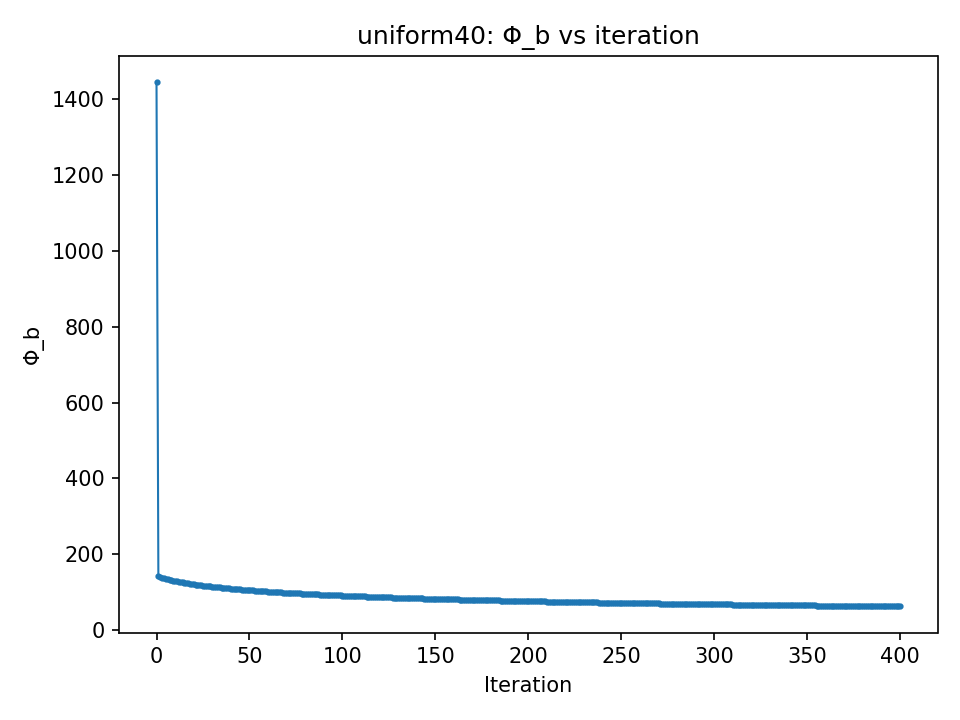
\includegraphics[width=0.32\linewidth]{figures/uniform40_dx0.01_phib_vs_iter.png}
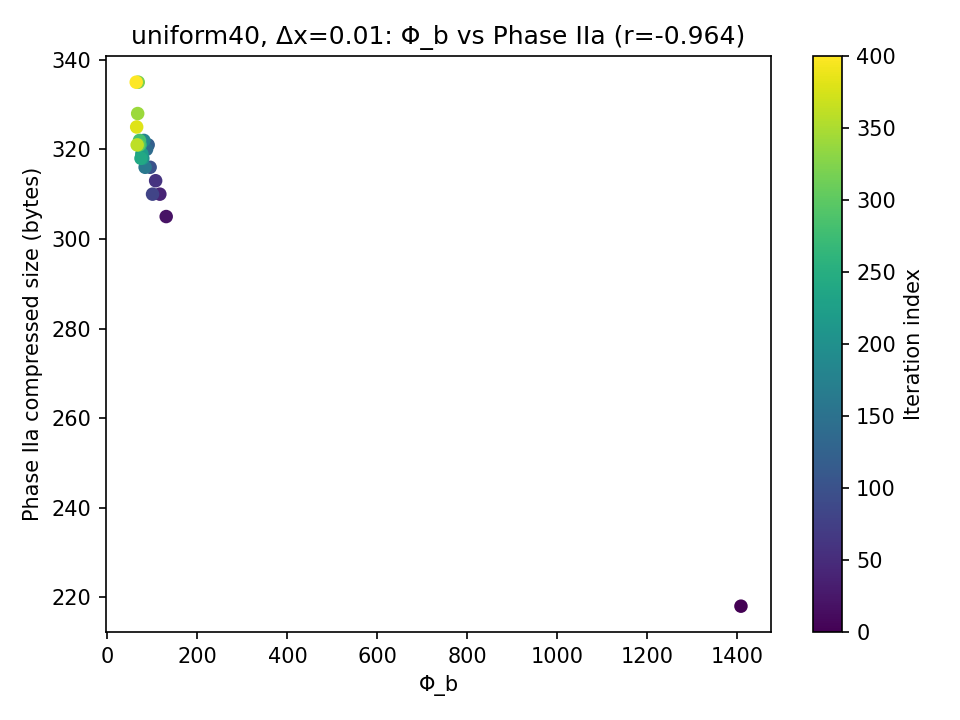
\includegraphics[width=0.32\linewidth]{figures/uniform40_dx0.01_phib_vs_phase2a.png}
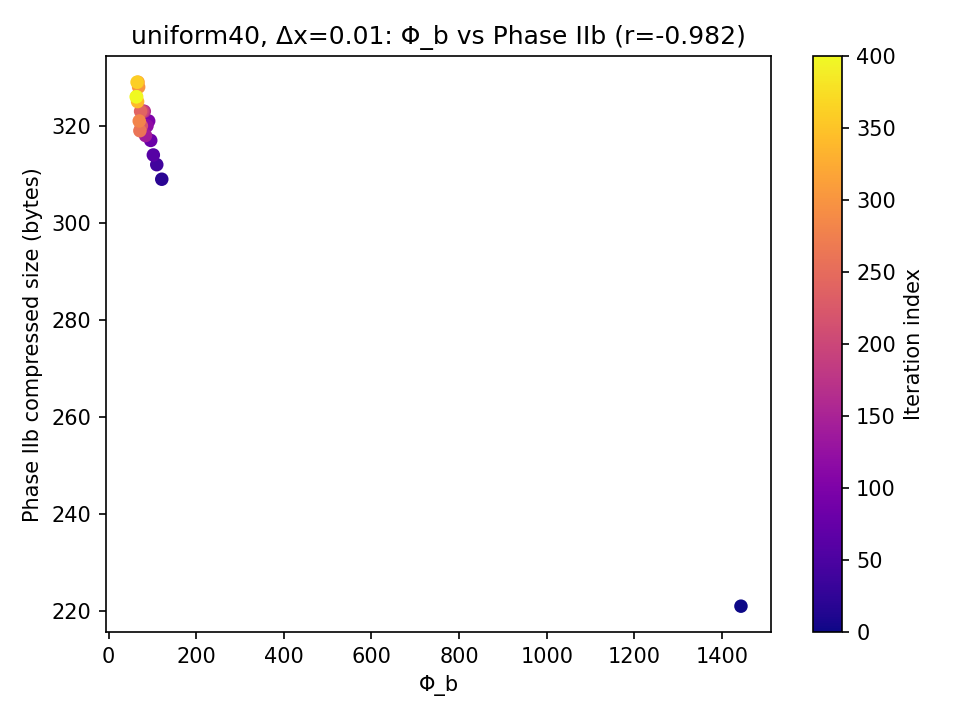
\includegraphics[width=0.32\linewidth]{figures/uniform40_dx0.01_phib_vs_phase2b.png}
\caption{\textbf{Uniform40} ($\Delta x{=}10^{-2}$).  
Monotone $\phib$ descent and strong $\phib$–compression correlation across Phase IIa and IIb.}
\label{fig:uniform40}
\end{figure}

\begin{figure}[htbp]
\centering
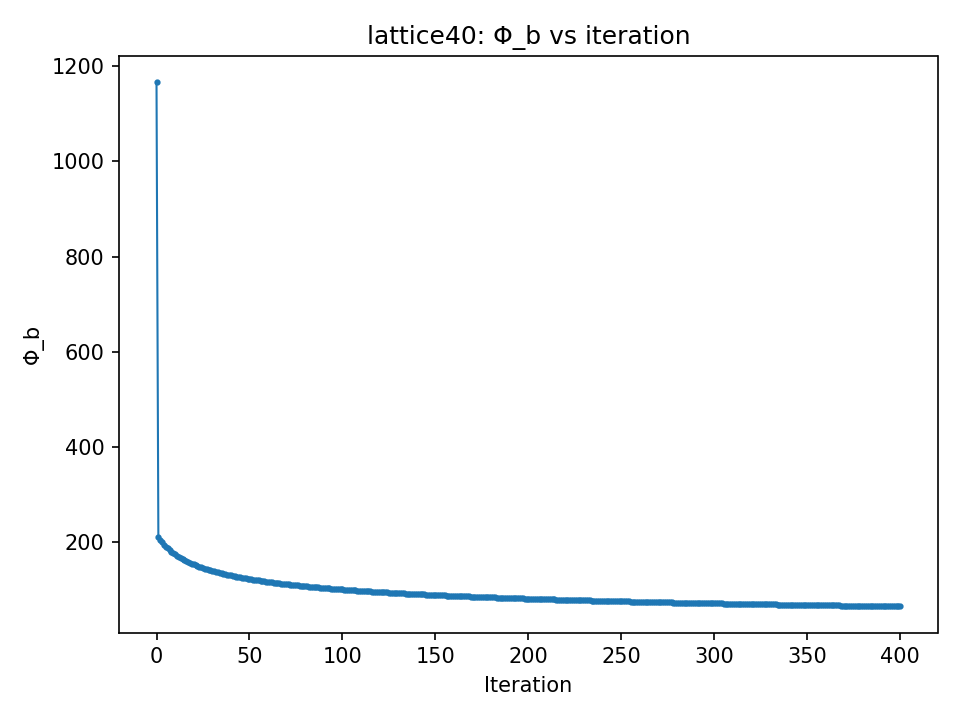
\includegraphics[width=0.32\linewidth]{figures/lattice40_dx0.01_phib_vs_iter.png}
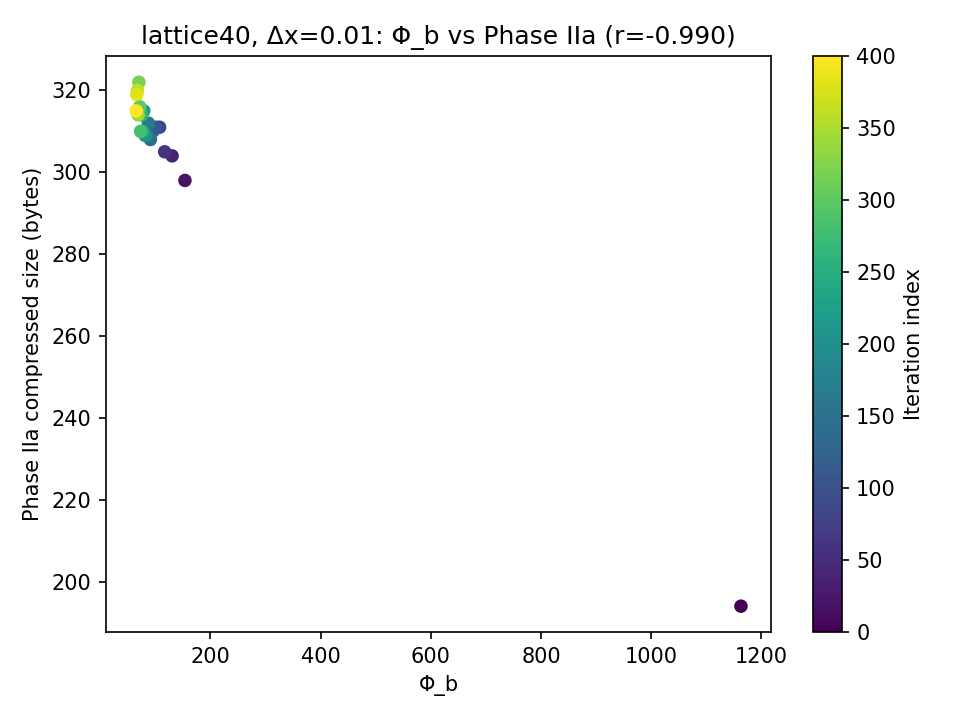
\includegraphics[width=0.32\linewidth]{figures/lattice40_dx0.01_phib_vs_phase2a.png}
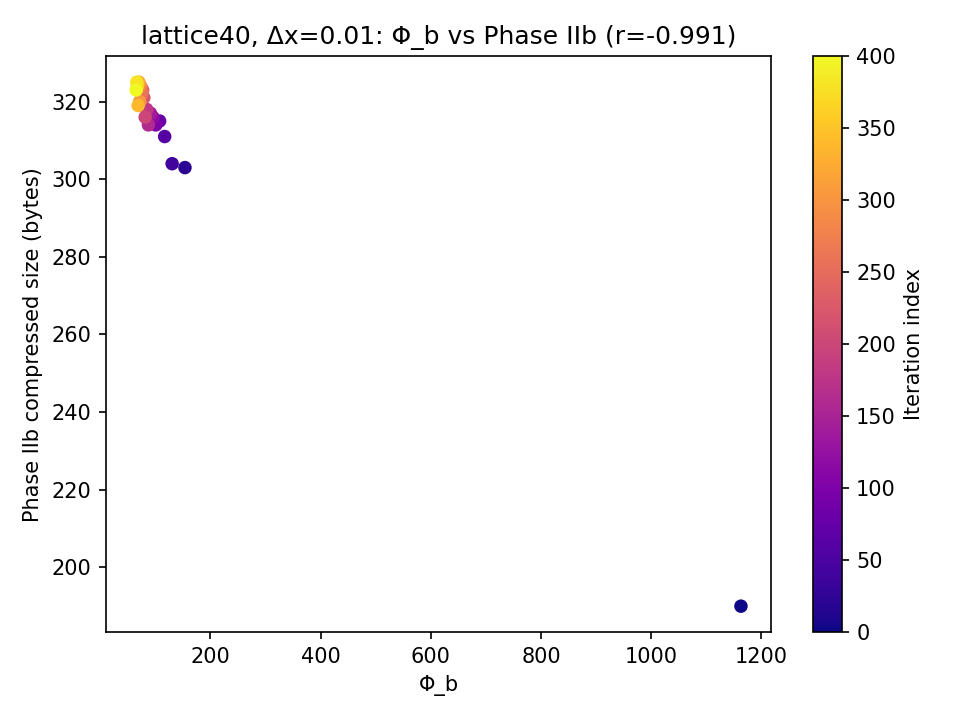
\includegraphics[width=0.32\linewidth]{figures/lattice40_dx0.01_phib_vs_phase2b.png}
\caption{\textbf{Lattice40} ($\Delta x{=}10^{-2}$).  
Plateaus indicate limited rearrangement; correlations weaker—rejection under F3.}
\label{fig:lattice40}
\end{figure}

\begin{figure}[htbp]
\centering
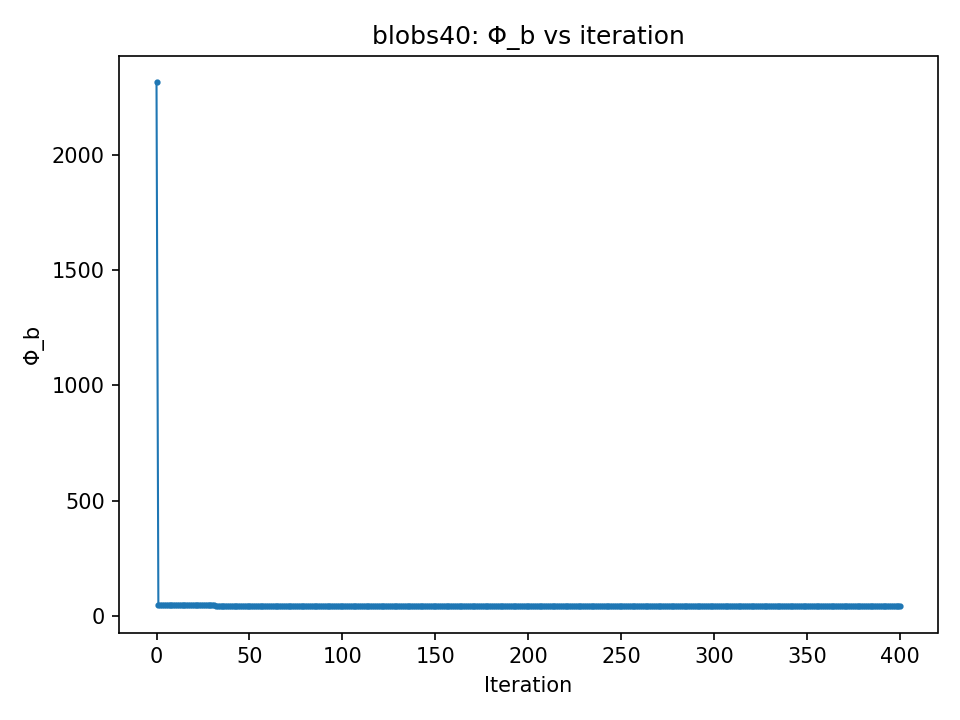
\includegraphics[width=0.32\linewidth]{figures/blobs40_dx0.01_phib_vs_iter.png}
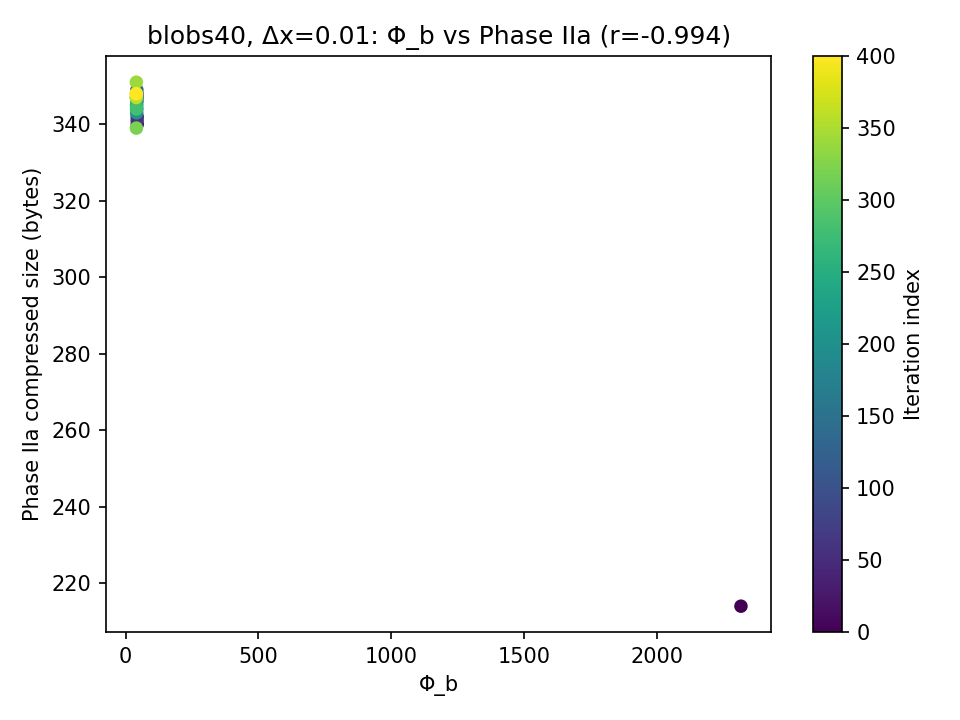
\includegraphics[width=0.32\linewidth]{figures/blobs40_dx0.01_phib_vs_phase2a.png}
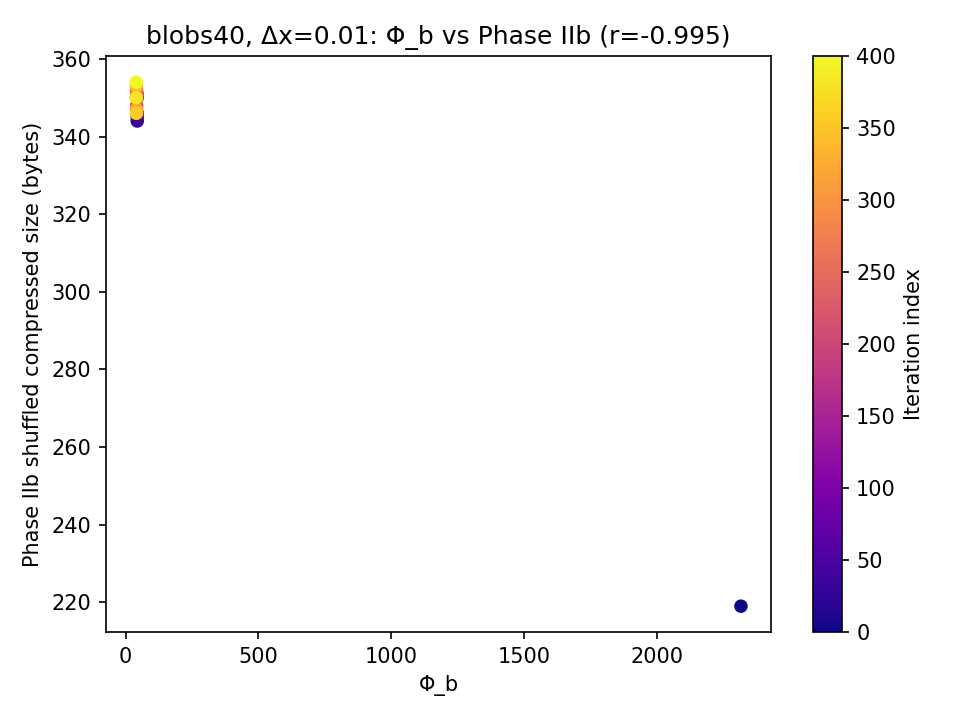
\includegraphics[width=0.32\linewidth]{figures/blobs40_dx0.01_phib_vs_phase2b.png}
\caption{\textbf{Blobs40} ($\Delta x{=}10^{-2}$).  
Strong monotone $\phib$–compression correlation; persistent across encoders.}
\label{fig:blobs40}
\end{figure}

\begin{figure}[htbp]
\centering
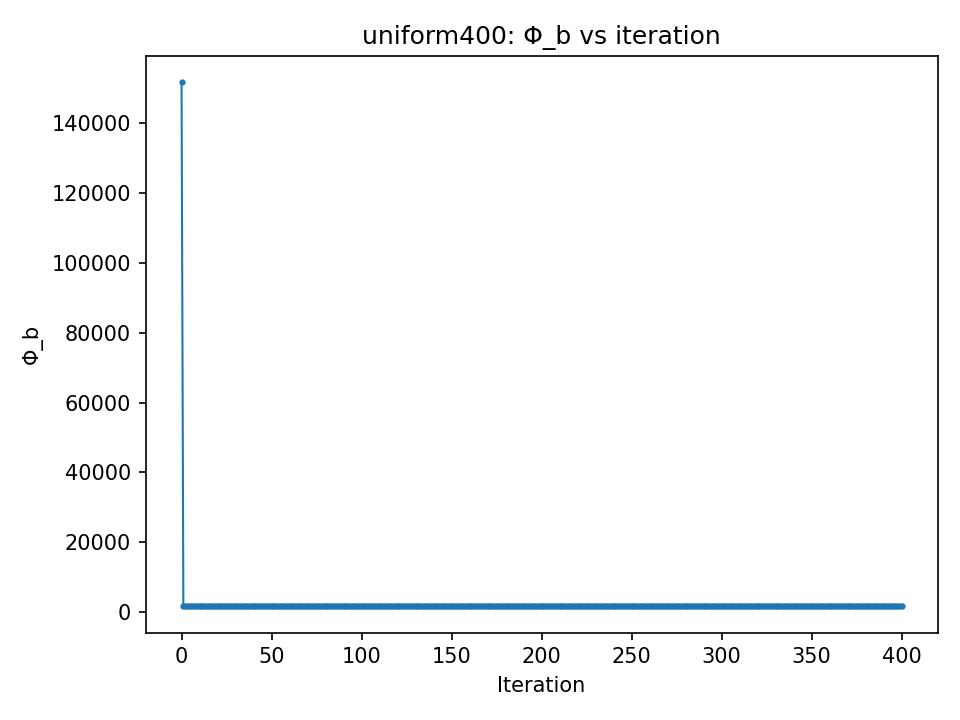
\includegraphics[width=0.32\linewidth]{figures/uniform400_dx0.001_phib_vs_iter.png}
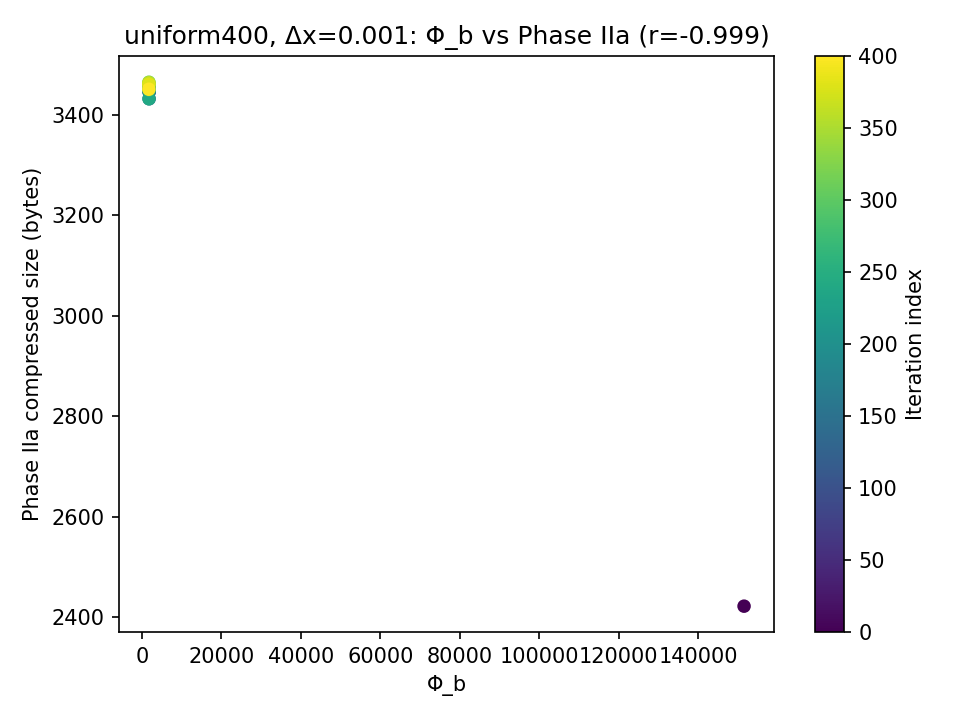
\includegraphics[width=0.32\linewidth]{figures/uniform400_dx0.001_phib_vs_phase2a.png}
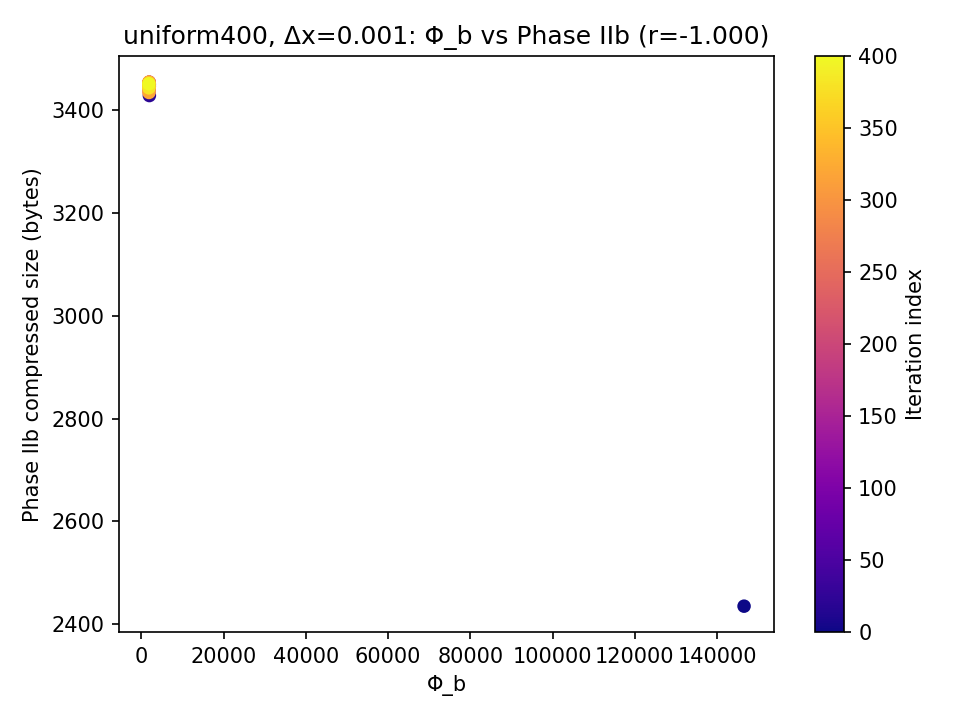
\includegraphics[width=0.32\linewidth]{figures/uniform400_dx0.001_phib_vs_phase2b.png}
\caption{\textbf{Uniform400} ($\Delta x{=}10^{-3}$).  
At scale, correlations approach $|r|\approx1$; stability across encoders and quantizations.}
\label{fig:uniform400}
\end{figure}

\section{Results and Interpretation}
$\phib$ decreases monotonically. In \texttt{uniform40}, \texttt{blobs40}, and \texttt{uniform400}, $\phib$ correlates strongly with compressed size under both coordinate encoders. In \texttt{lattice40}, correlations weaken—rejection under F3.  
For \texttt{uniform40} ($\Delta x=10^{-2}$), $\phib$ achieves $|r|\!\approx\!0.96$, exceeding geometric baselines ($0.74$–$0.89$).  
For $N{=}400$, all reach $|r|\!\approx\!1$.  
Decreasing $\phib$ sharpens spatial regularity; gzip exploits repeated integer triples after quantization. The effect persists under coordinate shuffling, demonstrating genuine spatial order.

\section{Model Card (Preregistered Parameters)}
\begin{itemize}
\item System: $N{=}40,400$, free boundaries, seed=0.
\item Functional: $\phib$ as in \cref{eq:phib-def}, $a{=}0.05$.
\item Update: Gradient descent with backtracking ($\eta_0{=}0.05$, shrink $0.5$, min $10^{-6}$).
\item Snapshots: every $5$ accepted steps.
\item Quantization: $\Delta x\in\{10^{-1},10^{-2},10^{-3}\}$.
\item Encoders: Phase I (64 radial bins + gzip), Phase IIa/IIb (quantized coords, gzip level 6).
\item Baselines: radius of gyration, mean NND, coordinate variance.
\item Falsifier: $|r|\ge0.7$ on subsampled snapshots.
\end{itemize}

\section{Limitations and Next Steps}
$n_\text{eff}\!\approx\!21$ is small; we report $r$ as an effect size only.  
Multiple seeds, bootstrap CIs, and higher-order surrogates are natural next steps.  
Phase IIb removes ordering bias but not all redundancy; future work could include PCA-based entropy estimators.

\section{Relation to Prior Work}
PCD unites:
\begin{itemize}
\item Gradient-flow methods (Fruchterman–Reingold–style);
\item Compression and MDL heuristics;
\item Explicit falsification in surrogate auditing.
\end{itemize}

\section{Conclusion}
PCD provides a minimal falsifiable loop:
\begin{enumerate}[label=(\arabic*)]
\item Choose $\phib$;
\item Evolve by monotone descent;
\item Measure compressed sizes (Phase I–IIb);
\item Sweep $\Delta x$;
\item Apply F3.
\end{enumerate}
Some ensembles pass, others fail—by design.  
A transparent, computable workflow for compression-pressure surrogates.

\section*{Acknowledgments}
We thank reviewers for insisting on external encoders, ordering control, quantization sweeps, baselines, temporal subsampling, and preregistration.  
Any remaining eccentricities are the author’s own—and Jeeves’s.

\bibliographystyle{plain}
\begin{thebibliography}{10}

\bibitem{Shannon1948}
C.~E. Shannon.
\newblock A mathematical theory of communication.
\newblock {\em Bell System Technical Journal}, 27:379--423, 623--656, 1948.

\bibitem{Rissanen1978}
J.~Rissanen.
\newblock Modeling by shortest data description.
\newblock {\em Automatica}, 14(5):465--471, 1978.

\bibitem{LeimkuhlerMatthews2016}
B.~Leimkuhler and C.~Matthews.
\newblock {\em Molecular Dynamics}.
\newblock Springer, 2016.

\bibitem{Wendland1995}
H.~Wendland.
\newblock Piecewise polynomial, positive definite and compactly supported radial functions.
\newblock {\em Adv. Comput. Math.}, 4:389--396, 1995.

\bibitem{FruchtermanReingold1991}
T.~M.~J. Fruchterman and E.~M. Reingold.
\newblock Graph drawing by force-directed placement.
\newblock {\em Software: Practice and Experience}, 21(11):1129--1164, 1991.

\end{thebibliography}

\end{document}
